\section*{Q1}
The default limitation of both stack size and maximum number of translation to 1 is very restrictive and so one expects to see a significant improvement in total log probability once either limit is increased. This proves to be true, but only in a very limited range for both variables, as illustrated in Figure 1.
\vspace{4mm} %4mm vertical space

Changing the maximum number of translations causes a sharp improvement, but it flattens out very quickly. The difference in total log probability between decoder with $k=10$ and $k=50$ is only 10\% of the difference between $k=1$ and $k=2$. No further improvements are observed for $k>50$.

Changing the stack size has a similar effect, although improvement tapers out even quicker. Increasing stack size to over 3 does not provide significant benefits.

Qualitatively, the difference between translations produced by the maximally limited system ($k=1$ and $s=1$) and one which produces the highest scoring output ($k=50$ and $s=10$) is that the latter text is more fluent and idiomatic, yet the meaning is equally difficult to grasp and there is no difference between the levels of syntactic correctness.

We did not investigate how parameter changes affect decoding speed. Simple timing methods seemed to be neither sensitive nor reliable enough to uncover any interesting trends for values of k and s in the range [1--100]. However, Figure 2 offers a decoding time comparison with the local reordering case. 
\vspace{4mm} %4mm vertical space

The following conclusions can be drawn:
\begin{enumerate}
	\item
	The intuitive insight that phrases can have multiple good translations, depending on the context, proves to be important. Increasing the maximum number of possible translations per phrase does improve output quality.
	\item
	The pruning heuristics used in decoding are justifiable, since the best translation can really be found by searching within the top few hypothesis in each stack. The best hypothesis is not always the very top one, as witnessed by the sharp increase in log probability when stack size is changed to 2, but it seems to almost always be one of the top 5 or so.
	\item
	There is a limit, and one that's quickly reached, to how good a monotonic decoder can perform. Allowing it to entertain more hypotheses cannot overcome inherent problems entailed by monotonicity.
\end{enumerate}

\begin{figure}
	\centering
	\begin{subfigure}{.8\linewidth}
		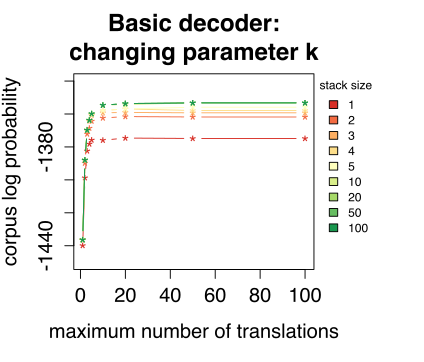
\includegraphics[scale=.75]{figures/d1_k.png}
		\caption{Increasing maximum number of translations, range [1--100].}
	\end{subfigure}
	\hskip2em
	\begin{subfigure}{.8\linewidth}
		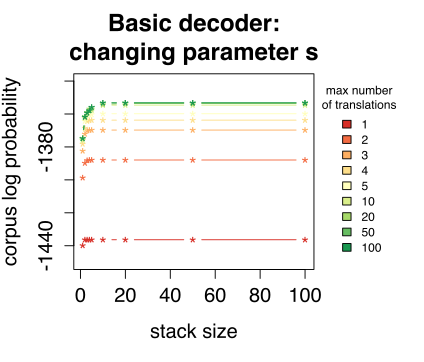
\includegraphics[scale=.75]{figures/d1_s.png}
		\caption{Increasing stack size, range [1--100].}
	\end{subfigure}
	\caption{Performance of decoder without reordering.}
\end{figure}
